\subsection{Futures}
\begin{frame}[fragile]{without Futures}
\begin{lstlisting}[frame=htrbl]
someCombinator :: [arr a b] -> [arr b c] -> arr [a] [c]
someCombinator fs1 fs2 =
	parEvalN () fs1 >>>	rightRotate >>>	parEvalN () fs2
\end{lstlisting}
\begin{center}
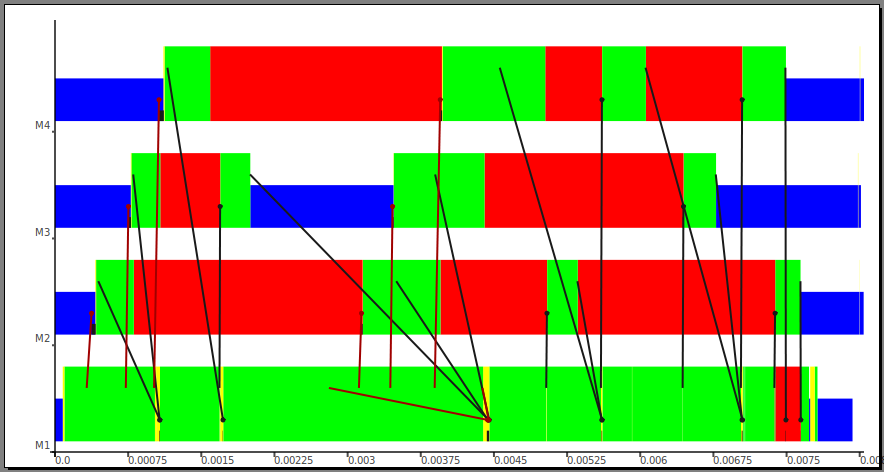
\includegraphics[scale=0.3]{images/withoutFutures}
\end{center}
\end{frame}
\begin{frame}[fragile]{with Futures}
\begin{lstlisting}[frame=htrbl]
someCombinator :: [arr a b] -> [arr b c] -> arr [a] [c]
someCombinator fs1 fs2 =
	parEvalN () (map (>>> put ()) fs1) >>>
	rightRotate >>>
	parEvalN () (map (get () >>>) fs2)
\end{lstlisting}
\begin{center}
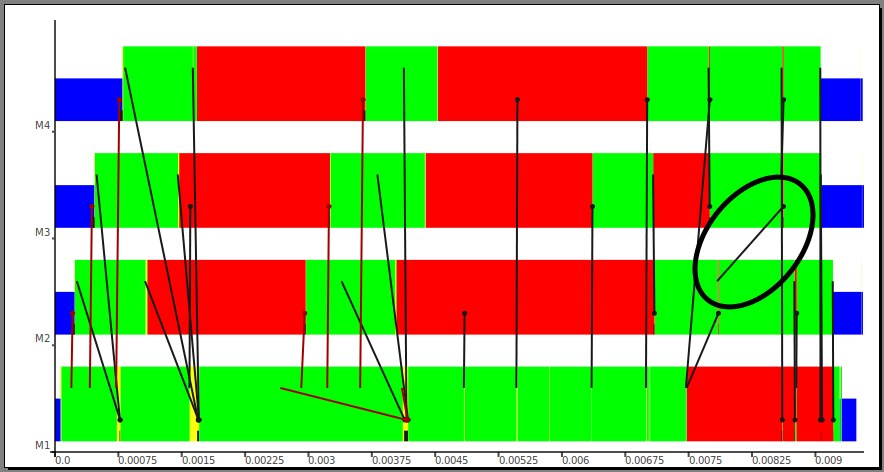
\includegraphics[scale=0.35]{images/withFutures}
\end{center}
\end{frame}